% !TEX spellcheck = en_US



% ~~~~~~~~~~~~~~~~~~~~~~~~~~~~~~~~~~~~~~~ V
% (NC) 2026 Haluk Bingol
% github.com/halukbingol/LaTeX-Templates
%
% Licensees may copy, distribute, display, and perform the work and make derivative works 
% and remixes based on it only for non-commercial purposes. 
% ~~~~~~~~~~~~~~~~~~~~~~~~~~~~~~~~~~~~~~~ A




% =====================================================================
%  Strings in Java -- Senior Level: Internals, Performance and Security
%  ---------------------------------------------------------------------
%  Built on hbCisLaTeXTemplate.tex with the libraries in ../../hblib/.
%  Programs and their outputs are read from codeoutput/:
%     codeoutput/<Name>.java   the program
%     codeoutput/<Name>.in     keyboard input (optional)
%     codeoutput/<Name>.txt    what it printed, made by:  sh run_examples.sh
% =====================================================================

\documentclass[aspectratio=169,10pt,compress]{beamer}

% ~~~~~~~~~~~~~~~~~~~~~~~~~~~~~~~~~~~~~~~~~~~~~~~~~~~~~~~~~~~~~~~~~ V hblib
	\usepackage{../../hblib/hblibPresentation} % lib presentation: theme, i/N, \hSection, algorithm2e, ...
	\usepackage{../../hblib/hblibCodeoutput} % lib code + output: \lstcode, \lstcodedown, ...
	\usepackage{../../hblib/hblibDatastructures} % lib data structures: \hString, \hStack, \hQueue
% ~~~~~~~~~~~~~~~~~~~~~~~~~~~~~~~~~~~~~~~~~~~~~~~~~~~~~~~~~~~~~~~~~ A hblib


% xcolor, array (and the L{width} column), listings, tikz and algorithm2e come from the hblib libraries
\usepackage[T1]{fontenc}
\usepackage{lmodern}
\usepackage{booktabs}

\definecolor{gitred}{RGB}{240,80,50}
\newcommand{\cmd}[1]{\texttt{\color{gitred}#1}}

% ---------------------------------------------------------------------
\title{Strings in Java}
\subtitle{Senior Level: Internals, Performance and Security}
\author[Bingol]{Haluk O. Bingol}

\institute[FCIS]{
    Faculty of Computer and Information Sciences\\
    Yeditepe University
}
\date{
	{\tiny \hbTimeStamp}
}

\begin{document}




% ~~~~~~~~~~~~~~~~~~~~~~~~~~~~~~~~~~~~~~ V frm
\begin{frame}[t,fragile]
  \titlepage
\end{frame}
% ~~~~~~~~~~~~~~~~~~~~~~~~~~~~~~~~~~~~~~ A frm




% ~~~~~~~~~~~~~~~~~~~~~~~~~~~~~~~~~~~~~~ V frm
\begin{frame}[t,fragile] \frametitle{Outline}
  \tableofcontents[hideallsubsections]
\end{frame}
% ~~~~~~~~~~~~~~~~~~~~~~~~~~~~~~~~~~~~~~ A frm

% ~~~~~~~~~~~~~~~~~~~~~~~~~~~~~~~~~~~~~~ V
\hSection[Inside]{Inside java.lang.String}{}{}
% ~~~~~~~~~~~~~~~~~~~~~~~~~~~~~~~~~~~~~~ A

% ~~~~~~~~~~~~~~~~~~~~~~~~~~~~~~~~~~~~~~ V
\subsection[Fields]{The fields}
% ~~~~~~~~~~~~~~~~~~~~~~~~~~~~~~~~~~~~~~ A




% ~~~~~~~~~~~~~~~~~~~~~~~~~~~~~~~~~~~~~~ V frm
\begin{frame}[t,fragile] \frametitle{What a \texttt{String} object holds (JDK 21)}
  \lstcoderightstep[0.62][basicstyle=\ttfamily\tiny][basicstyle=\ttfamily\scriptsize]{codeoutput/StringFields.java}{Java}{codeoutput/StringFields.txt}

  \vspace{0.3em}
  \small Found by reflection, without opening the class. Since Java 9 there is no \texttt{char[]}: the characters live in a
  \texttt{byte[]} plus a \texttt{coder} flag. \texttt{hash} caches \texttt{hashCode()}; \texttt{hashIsZero} (Java 13) avoids
  recomputing when the hash really is 0.
\end{frame}
% ~~~~~~~~~~~~~~~~~~~~~~~~~~~~~~~~~~~~~~ A frm

% ~~~~~~~~~~~~~~~~~~~~~~~~~~~~~~~~~~~~~~ V
\subsection[Compact]{Compact strings}
% ~~~~~~~~~~~~~~~~~~~~~~~~~~~~~~~~~~~~~~ A




% ~~~~~~~~~~~~~~~~~~~~~~~~~~~~~~~~~~~~~~ V frm
\begin{frame}[t,fragile] \frametitle{Compact strings (JEP 254, Java 9)}
  \begin{columns}[T]
    \begin{column}{0.52\textwidth}
      \small If every character fits in one byte (Latin-1, \texttt{U+0000}..\texttt{U+00FF}) the string is stored
      with \textbf{1 byte per char} (\texttt{coder = LATIN1}); otherwise \textbf{2 bytes per char} (\texttt{coder = UTF16}).
      \vspace{0.4em}

      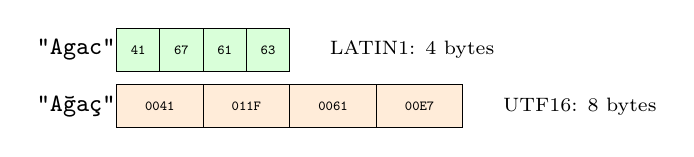
\begin{tikzpicture}[x=0.55cm, y=0.55cm, b/.style={draw, minimum size=0.55cm, font=\ttfamily\tiny, inner sep=0pt}]
        \node[anchor=east, font=\small] at (-0.3,0) {\texttt{"Agac"}};
        \foreach \v [count=\i from 0] in {41,67,61,63} \node[b, fill=green!15] at (\i,0) {\v};
        \node[anchor=west, font=\scriptsize] at (4.2,0) {LATIN1: 4 bytes};
        \node[anchor=east, font=\small] at (-0.3,-1.3) {\texttt{"Ağaç"}};
        \foreach \v [count=\i from 0] in {0041,011F,0061,00E7}
          \node[b, fill=orange!15, minimum width=1.1cm] at (2*\i+0.5,-1.3) {\v};
        \node[anchor=west, font=\scriptsize] at (8.2,-1.3) {UTF16: 8 bytes};
      \end{tikzpicture}

      \vspace{0.3em}
      \small \texttt{ç} (\texttt{E7}) alone would fit Latin-1; \texttt{ğ} (\texttt{011F}) does not, so the whole string is UTF16.
    \end{column}
    \begin{column}{0.44\textwidth}
      \begin{block}{Why it pays off}
        \small Most strings in real heaps (names, keys, JSON, logs) are Latin-1. Strings are often 25\%+ of the live heap,
        so halving their arrays saves real memory and cache bandwidth.
      \end{block}
      \begin{block}{Cost}
        \small A branch on \texttt{coder} in every operation; mixing coders (e.g.\ concatenating with \texttt{ğ}) inflates to UTF16.
      \end{block}
      \small The stack trace on the freshman slides showed it: \texttt{StringLatin1.charAt}.
    \end{column}
  \end{columns}
\end{frame}
% ~~~~~~~~~~~~~~~~~~~~~~~~~~~~~~~~~~~~~~ A frm




% ~~~~~~~~~~~~~~~~~~~~~~~~~~~~~~~~~~~~~~ V frm
\begin{frame}[t,fragile] \frametitle{Measuring it}
  \begin{columns}[T]
    \begin{column}{0.6\textwidth}
      \lstcode[basicstyle=\ttfamily\tiny]{codeoutput/CompactDemo.java}{Java}
      \lstcode[basicstyle=\ttfamily\tiny]{codeoutput/CompactStrings.sh}{bash}
    \end{column}
    \begin{column}{0.38\textwidth}
      \uncover<2->{\lstoutput[basicstyle=\ttfamily\tiny]{codeoutput/CompactStrings.txt}}
      \uncover<3->{
      \small One million 32-char strings: the \texttt{byte[]} needs 32 bytes instead of 64, plus a header,
      and each \texttt{String} object adds its own 24 bytes or so; hence about 30\% less, not 50\%.

      \vspace{0.3em}
      \hRemark{Rough numbers}: \texttt{totalMemory - freeMemory} after \texttt{System.gc()} is only an estimate;
      use JOL or a heap profiler for exact sizes.}
    \end{column}
  \end{columns}
\end{frame}
% ~~~~~~~~~~~~~~~~~~~~~~~~~~~~~~~~~~~~~~ A frm

% ~~~~~~~~~~~~~~~~~~~~~~~~~~~~~~~~~~~~~~ V
\hSection[JVM]{Strings and the JVM}{}{}
% ~~~~~~~~~~~~~~~~~~~~~~~~~~~~~~~~~~~~~~ A

% ~~~~~~~~~~~~~~~~~~~~~~~~~~~~~~~~~~~~~~ V
\subsection[Pool]{Pool and deduplication}
% ~~~~~~~~~~~~~~~~~~~~~~~~~~~~~~~~~~~~~~ A




% ~~~~~~~~~~~~~~~~~~~~~~~~~~~~~~~~~~~~~~ V frm
\begin{frame}[t,fragile] \frametitle{The string pool and deduplication}
  \begin{columns}[T]
    \begin{column}{0.48\textwidth}
      \begin{block}{The pool (\texttt{StringTable})}
        \small
        \begin{itemize}
          \item Literals and \texttt{intern()}ed strings live in a native hash table pointing into the heap
          \item In the main heap since Java 7 (before: PermGen), so pooled strings are garbage collected
          \item Size: \texttt{-XX:StringTableSize=N}; statistics: \cmd{jcmd <pid> VM.stringtable}
          \item \texttt{intern()} is a hash lookup; interning everything is rarely a win
        \end{itemize}
      \end{block}
    \end{column}
    \begin{column}{0.48\textwidth}
      \begin{block}{Deduplication (JEP 192)}
        \small
        \begin{itemize}
          \item \cmd{-XX:+UseStringDeduplication}: the GC finds strings with equal contents and lets them
                \textbf{share one} \texttt{byte[]}
          \item The \texttt{String} objects stay distinct, so \texttt{==} is unchanged
          \item First G1 only (Java 8u20); since Java 18 also Serial, Parallel and ZGC
          \item Good for heaps full of repeated values (CSV, JSON, database rows)
        \end{itemize}
      \end{block}
    \end{column}
  \end{columns}
  \vspace{0.2em}
  \small \hRemark{Windows and macOS alike}: \cmd{jps} lists running Java processes, \cmd{jcmd <pid> help} lists the commands;
  both are in the JDK's \texttt{bin} folder (Command Prompt or Terminal).
\end{frame}
% ~~~~~~~~~~~~~~~~~~~~~~~~~~~~~~~~~~~~~~ A frm

% ~~~~~~~~~~~~~~~~~~~~~~~~~~~~~~~~~~~~~~ V
\subsection[Indy]{Concatenation since Java 9}
% ~~~~~~~~~~~~~~~~~~~~~~~~~~~~~~~~~~~~~~ A




% ~~~~~~~~~~~~~~~~~~~~~~~~~~~~~~~~~~~~~~ V frm
\begin{frame}[t,fragile] \frametitle{What \texttt{+} compiles to (JEP 280)}
  \begin{columns}[T]
    \begin{column}{0.44\textwidth}
      \lstcode[basicstyle=\ttfamily\tiny]{codeoutput/Concat.java}{Java}
      \small \cmd{javap -c} disassembles (Windows and macOS alike); \texttt{Javap.sh} also uses
      \cmd{javac -XDstringConcat=inline}, the pre-Java-9 way.
      \vspace{0.3em}

      \uncover<3->{Java 9+: one \texttt{invokedynamic} to \texttt{makeConcatWithConstants}; the JVM chooses the
      strategy at run time. Old class files keep the \texttt{StringBuilder} chain: recompiling is a free speed-up.}
    \end{column}
    \begin{column}{0.54\textwidth}
      \uncover<2->{\lstoutput[basicstyle=\ttfamily\tiny]{codeoutput/Javap.txt}}
    \end{column}
  \end{columns}
\end{frame}
% ~~~~~~~~~~~~~~~~~~~~~~~~~~~~~~~~~~~~~~ A frm

% ~~~~~~~~~~~~~~~~~~~~~~~~~~~~~~~~~~~~~~ V
\subsection[Switch]{Switch on strings}
% ~~~~~~~~~~~~~~~~~~~~~~~~~~~~~~~~~~~~~~ A




% ~~~~~~~~~~~~~~~~~~~~~~~~~~~~~~~~~~~~~~ V frm
\begin{frame}[t,fragile] \frametitle{How \texttt{switch} on a string works}
  \begin{columns}[T]
    \begin{column}{0.4\textwidth}


% +++++++++++++++++++++++++++++++++++++++ V lst
%: -Lst.
\begin{lstlisting}[style=codesnippet, language=Java]
switch (cmd) {
    case "start" -> run();
    case "stop"  -> halt();
    default      -> help();
}
\end{lstlisting}
% +++++++++++++++++++++++++++++++++++++++ A lst



      \small Since Java 7. \texttt{javac} turns it into two switches.
    \end{column}
    \begin{column}{0.56\textwidth}


% +++++++++++++++++++++++++++++++++++++++ V lst
%: -Lst.
\begin{lstlisting}[style=codesnippet, language=Java, basicstyle=\ttfamily\scriptsize]
int k = -1;
switch (cmd.hashCode()) {          // 1: on the hash
    case 109757538:                // "start".hashCode()
        if (cmd.equals("start")) k = 0; break;
    case 3540994:                  // "stop".hashCode()
        if (cmd.equals("stop"))  k = 1; break;
}
switch (k) {                       // 2: on the index
    case 0 -> run();
    case 1 -> halt();
    default -> help();
}
\end{lstlisting}
% +++++++++++++++++++++++++++++++++++++++ A lst



    \end{column}
  \end{columns}
  \small Consequences: a \texttt{null} \texttt{cmd} throws \texttt{NullPointerException}; colliding hashes still work thanks to \texttt{equals};
  cost is one hash (cached) plus one \texttt{equals}.
\end{frame}
% ~~~~~~~~~~~~~~~~~~~~~~~~~~~~~~~~~~~~~~ A frm

% ~~~~~~~~~~~~~~~~~~~~~~~~~~~~~~~~~~~~~~ V
\hSection[Performance]{Performance}{}{}
% ~~~~~~~~~~~~~~~~~~~~~~~~~~~~~~~~~~~~~~ A

% ~~~~~~~~~~~~~~~~~~~~~~~~~~~~~~~~~~~~~~ V
\subsection[Benchmark]{Measuring correctly}
% ~~~~~~~~~~~~~~~~~~~~~~~~~~~~~~~~~~~~~~ A




% ~~~~~~~~~~~~~~~~~~~~~~~~~~~~~~~~~~~~~~ V frm
\begin{frame}[t,fragile] \frametitle{Benchmarking strings correctly}
  \begin{columns}[T]
    \begin{column}{0.52\textwidth}


% +++++++++++++++++++++++++++++++++++++++ V lst
%: -Lst.
\begin{lstlisting}[style=codesnippet, language=Java, basicstyle=\ttfamily\scriptsize]
@State(Scope.Benchmark)
public class ConcatBench {
    @Param({"10", "1000"}) int n;

    @Benchmark
    public String plus() {
        String s = "";
        for (int i = 0; i < n; i++) s += i;
        return s;              // keep the result alive
    }

    @Benchmark
    public String builder() {
        StringBuilder sb = new StringBuilder();
        for (int i = 0; i < n; i++) sb.append(i);
        return sb.toString();
    }
}
\end{lstlisting}
% +++++++++++++++++++++++++++++++++++++++ A lst



    \end{column}
    \begin{column}{0.44\textwidth}
      \small Hand-made timing (as in the sophomore slides) is fooled by
      \begin{itemize}\small
        \item JIT warm-up and on-stack replacement
        \item dead-code elimination of unused results
        \item constant folding, GC pauses, CPU frequency
      \end{itemize}
      Use \textbf{JMH} (Java Microbenchmark Harness):


% +++++++++++++++++++++++++++++++++++++++ V lst
%: -Lst.
\begin{lstlisting}[style=codesnippet, language=bash, basicstyle=\ttfamily\tiny]
mvn archetype:generate \
  -DarchetypeGroupId=org.openjdk.jmh \
  -DarchetypeArtifactId=jmh-java-benchmark-archetype
mvn package
java -jar target/benchmarks.jar
\end{lstlisting}
% +++++++++++++++++++++++++++++++++++++++ A lst



      \footnotesize Maven: macOS \cmd{brew install maven}; Windows: unzip from \texttt{maven.apache.org} and add \texttt{bin} to \texttt{PATH}.
      In Command Prompt write each command on one line (no \texttt{\textbackslash}).
    \end{column}
  \end{columns}
\end{frame}
% ~~~~~~~~~~~~~~~~~~~~~~~~~~~~~~~~~~~~~~ A frm

% ~~~~~~~~~~~~~~~~~~~~~~~~~~~~~~~~~~~~~~ V
\subsection[Guide]{Guidelines}
% ~~~~~~~~~~~~~~~~~~~~~~~~~~~~~~~~~~~~~~ A




% ~~~~~~~~~~~~~~~~~~~~~~~~~~~~~~~~~~~~~~ V frm
\begin{frame}[t,fragile] \frametitle{Performance guidelines}
  \small
  \begin{tabular}{@{}L{0.44\textwidth}L{0.5\textwidth}@{}}
    \toprule
    \textbf{Do} & \textbf{Why} \\
    \midrule
    \texttt{+} for a few pieces in one expression        & compiled to one optimized \texttt{invokedynamic} \\
    \texttt{StringBuilder} (presized) in loops            & avoids $O(n^{2})$ copying and regrowth \\
    \texttt{String.join}, \texttt{Collectors.joining}     & clear and already efficient \\
    \texttt{Pattern.compile} once, reuse                  & \texttt{s.matches(re)} recompiles every call \\
    \texttt{split} with a single plain char               & fast path without the regex engine \\
    \texttt{toLowerCase(Locale.ROOT)} for keys            & correct and locale-independent \\
    \texttt{equals} before \texttt{intern}                & interning costs a global table lookup \\
    \texttt{-XX:+UseStringDeduplication} for repetitive heaps & measured memory win, no code change \\
    \bottomrule
  \end{tabular}

  \vspace{0.4em}
  \hRemark{First measure, then optimize}: most string code is not the bottleneck.
\end{frame}
% ~~~~~~~~~~~~~~~~~~~~~~~~~~~~~~~~~~~~~~ A frm

% ~~~~~~~~~~~~~~~~~~~~~~~~~~~~~~~~~~~~~~ V
\subsection[API]{The modern API}
% ~~~~~~~~~~~~~~~~~~~~~~~~~~~~~~~~~~~~~~ A




% ~~~~~~~~~~~~~~~~~~~~~~~~~~~~~~~~~~~~~~ V frm
\begin{frame}[t,fragile] \frametitle{The modern \texttt{String} API (Java 11--21)}
  \lstcodeoverlaystep[basicstyle=\ttfamily\tiny][basicstyle=\ttfamily\tiny][0.28\textwidth]{11.0cm,2.25cm}{codeoutput/ModernApi.java}{Java}{codeoutput/ModernApi.txt}

  \vspace{0.2em}
  \small The comment on each line is the Java version that added the method.
\end{frame}
% ~~~~~~~~~~~~~~~~~~~~~~~~~~~~~~~~~~~~~~ A frm

% ~~~~~~~~~~~~~~~~~~~~~~~~~~~~~~~~~~~~~~ V
\hSection[Security]{Security}{}{}
% ~~~~~~~~~~~~~~~~~~~~~~~~~~~~~~~~~~~~~~ A

% ~~~~~~~~~~~~~~~~~~~~~~~~~~~~~~~~~~~~~~ V
\subsection[Passwords]{Passwords}
% ~~~~~~~~~~~~~~~~~~~~~~~~~~~~~~~~~~~~~~ A




% ~~~~~~~~~~~~~~~~~~~~~~~~~~~~~~~~~~~~~~ V frm
\begin{frame}[t,fragile] \frametitle{Secrets do not belong in a \texttt{String}}
  \begin{columns}[T]
    \begin{column}{0.5\textwidth}


% +++++++++++++++++++++++++++++++++++++++ V lst
%: -Lst.
\begin{lstlisting}[style=codesnippet, language=Java]
char[] pw = System.console()
        .readPassword("Password: ");
try {
    authenticate(pw);
} finally {
    Arrays.fill(pw, ' ');  // wipe
}
\end{lstlisting}
% +++++++++++++++++++++++++++++++++++++++ A lst



      \small \texttt{Console.readPassword} does not echo and returns \texttt{char[]};
      \texttt{PBEKeySpec} and \texttt{KeyStore} also take \texttt{char[]}.
    \end{column}
    \begin{column}{0.46\textwidth}
      \small A password in a \texttt{String}
      \begin{itemize}\small
        \item cannot be wiped (immutable)
        \item stays in the heap until GC, maybe longer; may be pooled or deduplicated
        \item shows up in heap dumps, core files and \texttt{toString()} logs
      \end{itemize}
      \begin{alertblock}{Honest limits}
        \small Copies made by the GC or by libraries can survive the wipe. It reduces the exposure window; it is not a guarantee.
      \end{alertblock}
    \end{column}
  \end{columns}
\end{frame}
% ~~~~~~~~~~~~~~~~~~~~~~~~~~~~~~~~~~~~~~ A frm

% ~~~~~~~~~~~~~~~~~~~~~~~~~~~~~~~~~~~~~~ V
\subsection[Injection]{Injection}
% ~~~~~~~~~~~~~~~~~~~~~~~~~~~~~~~~~~~~~~ A




% ~~~~~~~~~~~~~~~~~~~~~~~~~~~~~~~~~~~~~~ V frm
\begin{frame}[t,fragile] \frametitle{Building queries from strings}
  \lstcodedownstep[basicstyle=\ttfamily\scriptsize][basicstyle=\ttfamily\tiny]{codeoutput/Injection.java}{Java}{codeoutput/Injection.txt}

  \small Concatenated input becomes \textbf{code}: the condition is always true. With \texttt{PreparedStatement}
  (\texttt{ps.setString(1, user)}) the input stays \textbf{data}. The same holds for shell commands, HTML (XSS),
  file paths (\texttt{../}) and log lines (newlines): \hRemark{never splice untrusted text into a language}.
\end{frame}
% ~~~~~~~~~~~~~~~~~~~~~~~~~~~~~~~~~~~~~~ A frm

% ~~~~~~~~~~~~~~~~~~~~~~~~~~~~~~~~~~~~~~ V
\subsection[Locale]{The Turkish locale bug}
% ~~~~~~~~~~~~~~~~~~~~~~~~~~~~~~~~~~~~~~ A




% ~~~~~~~~~~~~~~~~~~~~~~~~~~~~~~~~~~~~~~ V frm
\begin{frame}[t,fragile] \frametitle{The Turkish \texttt{i} as a security bug}
  \lstcoderightstep[0.66][basicstyle=\ttfamily\tiny][basicstyle=\ttfamily\tiny]{codeoutput/LocaleBug.java}{Java}{codeoutput/LocaleBug.txt}

  \vspace{0.3em}
  \small With a Turkish default locale the check silently fails and \texttt{"FILE".toLowerCase()} is \texttt{"fıle"}
  (keywords, file extensions, HTTP headers). \hRemark{Always pass} \texttt{Locale.ROOT} for machine-readable text.
\end{frame}
% ~~~~~~~~~~~~~~~~~~~~~~~~~~~~~~~~~~~~~~ A frm

% ~~~~~~~~~~~~~~~~~~~~~~~~~~~~~~~~~~~~~~ V
\subsection[ReDoS]{Regular expression denial of service}
% ~~~~~~~~~~~~~~~~~~~~~~~~~~~~~~~~~~~~~~ A




% ~~~~~~~~~~~~~~~~~~~~~~~~~~~~~~~~~~~~~~ V frm
\begin{frame}[t,fragile] \frametitle{Catastrophic backtracking (ReDoS)}
  \lstcoderightstep[0.62][basicstyle=\ttfamily\tiny][basicstyle=\ttfamily\tiny]{codeoutput/ReDoS.java}{Java}{codeoutput/ReDoS.txt}

  \vspace{0.3em}
  \small Java 21 handles the textbook \texttt{(a+)+b}, but \texttt{(.*a)\{20\}} grows 5 to $10\times$ per 4 characters;
  the unambiguous rewrite accepts the same strings in microseconds. \hRemark{Limit untrusted regexes and inputs.}
\end{frame}
% ~~~~~~~~~~~~~~~~~~~~~~~~~~~~~~~~~~~~~~ A frm

% ~~~~~~~~~~~~~~~~~~~~~~~~~~~~~~~~~~~~~~ V
\subsection[Hash flood]{Hash flooding}
% ~~~~~~~~~~~~~~~~~~~~~~~~~~~~~~~~~~~~~~ A




% ~~~~~~~~~~~~~~~~~~~~~~~~~~~~~~~~~~~~~~ V frm
\begin{frame}[t,fragile] \frametitle{Hash flooding: many keys, one hash}
  \lstcodeoverlaystep[basicstyle=\ttfamily\tiny][basicstyle=\ttfamily\tiny][0.3\textwidth]{10.9cm,2.25cm}{codeoutput/HashFlood.java}{Java}{codeoutput/HashFlood.txt}

  \vspace{0.2em}
  \small Java 8+ (JEP 180): a crowded bucket becomes a tree ordered by \texttt{compareTo}, $O(\log n)$ per operation.
\end{frame}
% ~~~~~~~~~~~~~~~~~~~~~~~~~~~~~~~~~~~~~~ A frm

% ~~~~~~~~~~~~~~~~~~~~~~~~~~~~~~~~~~~~~~ V
\hSection[Evolution]{Evolution of Strings in Java}{}{}
% ~~~~~~~~~~~~~~~~~~~~~~~~~~~~~~~~~~~~~~ A

% ~~~~~~~~~~~~~~~~~~~~~~~~~~~~~~~~~~~~~~ V
\subsection[Timeline]{Timeline}
% ~~~~~~~~~~~~~~~~~~~~~~~~~~~~~~~~~~~~~~ A




% ~~~~~~~~~~~~~~~~~~~~~~~~~~~~~~~~~~~~~~ V frm
\begin{frame}[t,fragile] \frametitle{Timeline}
  \footnotesize
  \begin{tabular}{@{}L{0.12\textwidth}L{0.82\textwidth}@{}}
    \toprule
    \textbf{Java} & \textbf{String-related change} \\
    \midrule
    1.0 (1996)  & \texttt{String}, synchronized \texttt{StringBuffer} \\
    5 (2004)    & \texttt{StringBuilder} (unsynchronized), \texttt{String.format}, code-point methods \\
    7 (2011)    & \texttt{switch} on strings; pool moved to the heap; \texttt{substring} copies (7u6) \\
    8 (2014)    & \texttt{String.join}, \texttt{chars()}; \texttt{HashMap} tree bins (JEP 180) \\
    9 (2017)    & compact strings (JEP 254); \texttt{invokedynamic} concatenation (JEP 280) \\
    11 (2018)   & \texttt{isBlank}, \texttt{lines}, \texttt{strip}, \texttt{repeat} \\
    15 (2020)   & text blocks (JEP 378), \texttt{formatted}, \texttt{stripIndent} \\
    18 (2022)   & UTF-8 by default (JEP 400); string deduplication in all collectors \\
    21 (2023)   & \texttt{splitWithDelimiters}, \texttt{StringBuilder.repeat}; string templates as a \emph{preview} (JEP 430) \\
    23 (2024)   & string templates \textbf{withdrawn} for redesign: a reminder that previews can disappear \\
    \bottomrule
  \end{tabular}
\end{frame}
% ~~~~~~~~~~~~~~~~~~~~~~~~~~~~~~~~~~~~~~ A frm

% ~~~~~~~~~~~~~~~~~~~~~~~~~~~~~~~~~~~~~~ V
\hSection[Summary]{Summary}{}{}
% ~~~~~~~~~~~~~~~~~~~~~~~~~~~~~~~~~~~~~~ A

% ~~~~~~~~~~~~~~~~~~~~~~~~~~~~~~~~~~~~~~ V
\subsection[Takeaways]{Takeaways}
% ~~~~~~~~~~~~~~~~~~~~~~~~~~~~~~~~~~~~~~ A




% ~~~~~~~~~~~~~~~~~~~~~~~~~~~~~~~~~~~~~~ V frm
\begin{frame}[t,fragile] \frametitle{Takeaways}
  \begin{columns}[T]
    \begin{column}{0.48\textwidth}
      \begin{block}{Internals}
        \small \texttt{byte[]} + \texttt{coder}; cached hash; pool in the heap; deduplication by the GC;
        \texttt{+} is an \texttt{invokedynamic} call site.
      \end{block}
      \begin{block}{Performance}
        \small Measure with JMH. \texttt{StringBuilder} in loops, compiled \texttt{Pattern}s, \texttt{Locale.ROOT},
        no premature \texttt{intern}.
      \end{block}
    \end{column}
    \begin{column}{0.48\textwidth}
      \begin{alertblock}{Security}
        \small Secrets in \texttt{char[]}; parameters, not concatenation; \texttt{Locale.ROOT} in checks;
        bounded, unambiguous regexes; expect colliding keys.
      \end{alertblock}
      \begin{block}{Portability}
        \small Explicit UTF-8 everywhere; normalize before comparing; test with Turkish and non-BMP text on
        Windows \emph{and} macOS.
      \end{block}
    \end{column}
  \end{columns}
\end{frame}
% ~~~~~~~~~~~~~~~~~~~~~~~~~~~~~~~~~~~~~~ A frm

% ~~~~~~~~~~~~~~~~~~~~~~~~~~~~~~~~~~~~~~ V
\subsection[Projects]{Projects}
% ~~~~~~~~~~~~~~~~~~~~~~~~~~~~~~~~~~~~~~ A




% ~~~~~~~~~~~~~~~~~~~~~~~~~~~~~~~~~~~~~~ V frm
\begin{frame}[t,fragile] \frametitle{Projects}
  \begin{enumerate}\small
    \item With JMH, compare \texttt{+}, \texttt{StringBuilder}, \texttt{String.join} and \texttt{Collectors.joining}
          for 10 to $10^{6}$ parts; explain the curves.
    \item Measure the heap of a CSV loader with and without \texttt{-XX:+UseStringDeduplication} (use \cmd{jcmd <pid> GC.heap\_info}).
    \item Use JOL (Java Object Layout) to print the exact size of \texttt{"Agac"} and \texttt{"Ağaç"}.
    \item Write a linter that flags \texttt{toUpperCase()}/\texttt{toLowerCase()} calls without a \texttt{Locale}.
    \item Build a regex sandbox that rejects patterns or inputs that run longer than 50\,ms
          (hint: a \texttt{CharSequence} wrapper whose \texttt{charAt} checks a deadline).
    \item Implement a rope (a tree of string pieces) with $O(\log n)$ insert; compare with \texttt{StringBuilder.insert}.
  \end{enumerate}
\end{frame}
% ~~~~~~~~~~~~~~~~~~~~~~~~~~~~~~~~~~~~~~ A frm




% ~~~~~~~~~~~~~~~~~~~~~~~~~~~~~~~~~~~~~~ V frm
\begin{frame}[t,fragile]
	\begin{center}
		\vspace{4cm}
		\hRemark{\Huge Questions?}
	\end{center}
\end{frame}
% ~~~~~~~~~~~~~~~~~~~~~~~~~~~~~~~~~~~~~~ A frm



\end{document}
